\documentclass[12pt, letterpaper, notitlepage, DIV=16, BCOR=1mm, headlines=2]{scrreprt}

\usepackage[hidelinks]{hyperref}
\usepackage[T1]{fontenc}
\usepackage{mathptmx}
\usepackage{graphicx}
\usepackage{siunitx}
%\graphicspath{{../}}

% make it a little easier on the eyes (next three line dark mode)
%\usepackage{xcolor}
%\pagecolor[rgb]{0,0,0} %black
%\color[rgb]{0.75,0.75,0.75} %grey

% make the default font times new roman
\setkomafont{disposition}{\rmfamily}

% make sure title and toc are on same page
\makeatletter
\newcommand*{\tocontents}{\@starttoc{toc}}
\makeatother

% add hyperlinks to toc
\hypersetup{
  linktoc=all
}

% adjust chapter height
\RedeclareSectionCommand[beforeskip=0pt]{chapter}

% remove page break before chapter titles
%\RedeclareSectionCommand[style=section]{chapter}

\title{AnalogIC Assignment 1}
\author{William Daniel Hiromoto}
\date{\today}

\begin{document}

\maketitle
%\tocontents{}

\begin{figure}[h]
	\makebox[\textwidth]{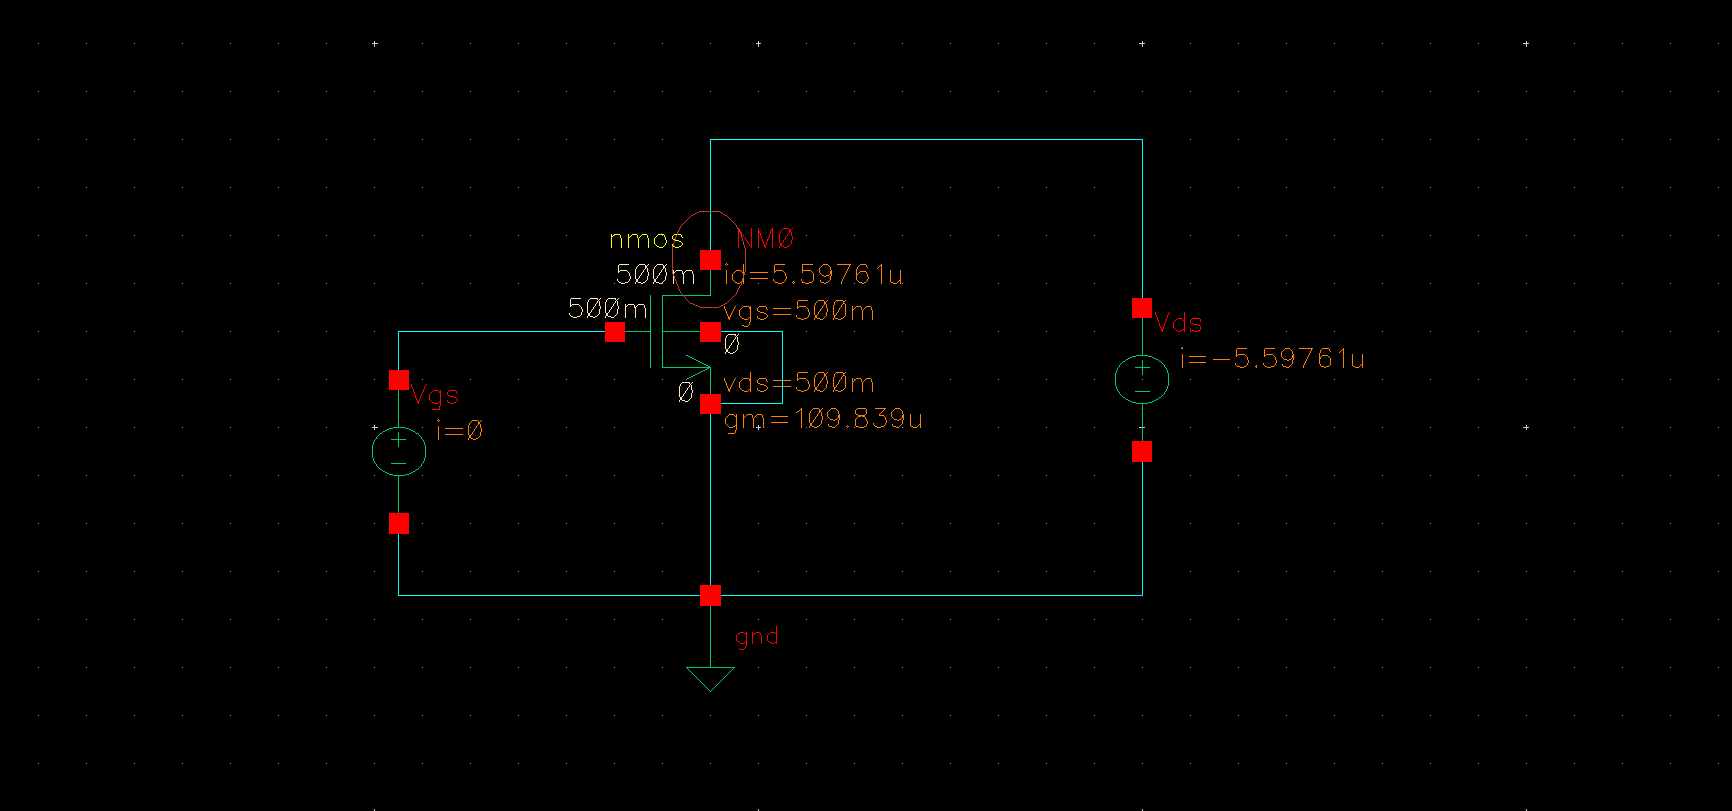
\includegraphics[width=\textwidth]{../Schematic.png}}
	\caption{Schematic from Cadence with DC annotations where nmos transistor dimensions are $W = 3\mu m$ and $L = 0.24\mu m$}
	\label{fig:Schematic}
\end{figure}

\pagebreak
\section*{Question 1}

\begin{figure}[h]
	\makebox[\textwidth]{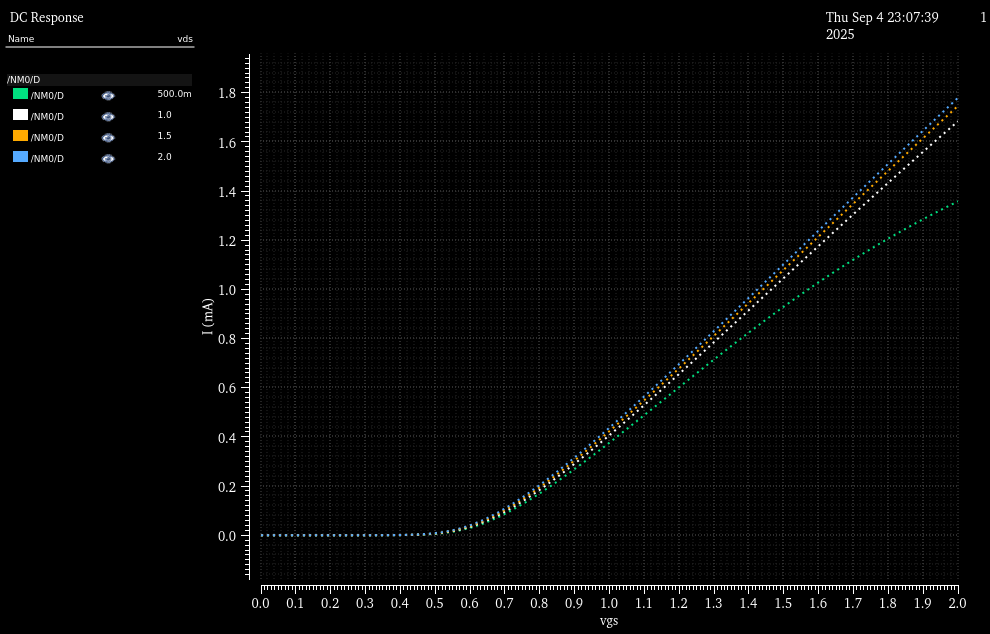
\includegraphics[width=\textwidth]{../Q1.png}}
	\caption{$V_{gs}$ sweep from $0V-2V$ for $V_{ds}= 0.5V, 1V, 1.5V,$ and $2V$}
	\label{fig:q1}
\end{figure}

Based on fig. \ref{fig:q1},
it would seam the minimum operating voltage of $V_{ds}$ for the transistor would be $0.5V$. At $V_{ds} = 0.5V$, 
while the transistor might still be able to run, the current is not able to rise as high as $V_{ds}$ 
at higher voltages. If the sweep was done with a larger maximum, it is likely that the transistor would
enter the linear region at a lower voltage for $V_{gs}$.

\pagebreak
\section*{Question 2a}

Based on the results found in fig. \ref{fig:q2a},
the transistor needs to have a $V_{gs} > 0.5V$ to reach its saturation point. $0.5V$ would 
then be the value for $V_{th}$. However, the current running through the transistor at $0.5V$ is on
the scale of less than 10 micro Amps.

\begin{figure}[ht]
	\makebox[\textwidth]{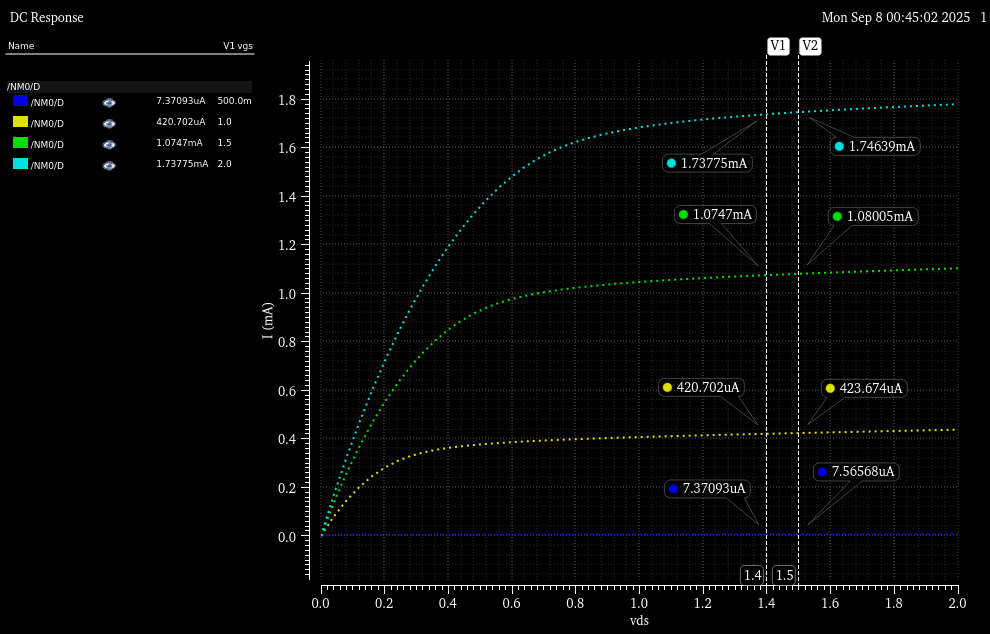
\includegraphics[width=\textwidth]{../Q2a.png}}
	\caption{$V_{ds}$ sweep from $0V-2V$ for $V_{gs}= 0.5V, 1V, 1.5V,$ and $2V$}
	\label{fig:q2a}
\end{figure}

\subsection*{2b}

The output resistance of a mosfet transistor is approximately given by 
$R_{out} \approx \frac{1}{\lambda I_d}$.
Cadence will provide the output conductance
$g_{ds} = \lambda I_d$ 
value after requesting the results of a simulation and selecting the transistor.
In both cases, to find the approximate value of the output resistance, the channel-length
modulation coefficient ($\lambda $) needs to be found. With the transistor in saturation,
the current becomes a function of the $V_{ds}$ in the sweep:

$$
I_d = \frac{1}{2}\mu _n C_{ox}\frac{W}{L}(V_{gs}-V_{th})^2 (1+\lambda V_{ds})
$$

If we pick two points and take the ratio of two points on the line in the linear region:

$$
\frac{I_{d1}}{I_{d2}} = \frac{(1+\lambda V_{ds1})}{(1+\lambda V_{ds2})}
$$
$$
\lambda = \frac{I_{d2}-I_{d1}}{V_{ds2}I_{d1}-V_{ds1}I_{d2}}
%\frac{420.720 \mu A}{423.674 \mu A} = \frac{(1+\lambda 1.4V)}{(1+\lambda 1.5V)}
$$

As the $\lambda $ will change with different values of $V_{gs}$ (and thus the output resistance).
As a result, the output resistance will be found using the simulation for $V_{gs} = 1V$.

$$
\lambda = \frac{432.674\mu A - 420.702\mu A}{1.5V \times 420.702\mu A - 1.4V \times 432.674\mu A}
= 0.473
$$
$$
R_{out} \approx \frac{1}{0.473 \times 432.674} \approx 4886.276
$$

\pagebreak
\begin{figure}[!ht]
	\makebox[\textwidth]{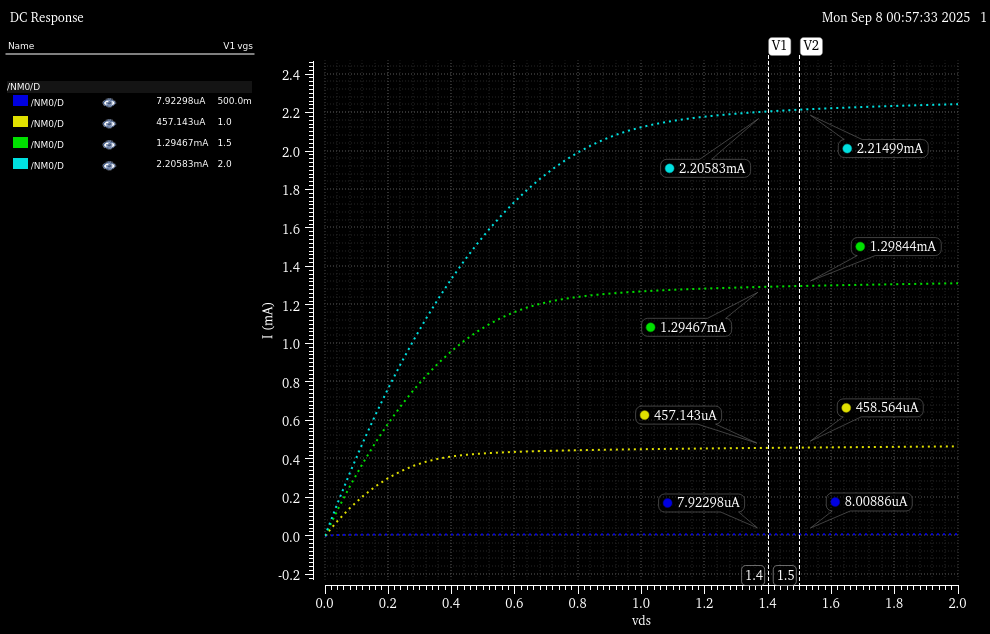
\includegraphics[width=\textwidth]{../Q2c.png}}
	\caption{Circuit from fig. \ref{fig:q2a} 
  but with $w = 6\mu m$ and $L = 0.48\mu m$ (dimensions doubled)}
	\label{fig:q2c}
\end{figure}
\subsection*{2c}

Retrying the same formula as 2b and $V_{gs} = 1V$:
$$
\lambda = \frac{458.564\mu A - 457.143\mu A}{1.5V \times 457.143\mu A - 1.4V \times 458.564\mu A}
= 0.0324
$$
$$
R_{out} \approx \frac{1}{0.0324 \times 458.564} \approx 67306.193
$$

Based on the results, with a doubling of the transistor dimensions, it seems that the output
resistance has grown exponentially. Generally, signal strength decreases exponentially over distances,
and assuming that a larger transistor size would mean the electrons would have to travel a larger distance,
it would make sense the resistance would be exponentially larger.

\pagebreak
\section*{Question 3a}
\begin{figure}[!ht]
	\makebox[\textwidth]{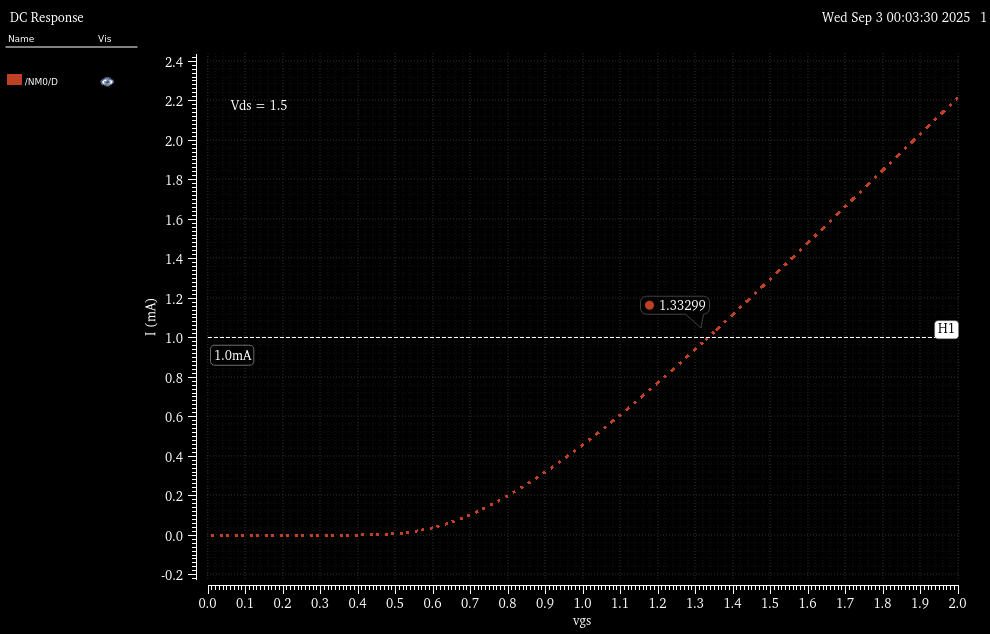
\includegraphics[width=\textwidth]{../Q3a.png}}
	\caption{$V_{gs}$ Sweep done on transistor from fig. \ref{fig:q2c}
  with $V_{ds} = 1.5V$. $1.0mA$ horizontal line and intersection marked}
	\label{fig:q3a}
\end{figure}

From the simulation, a voltage of approximately $V_{gs} = 1.33299V$ at $V_{ds} = 1.5V$ would be required
to reach a 1mA drain current. The effective voltage would be:

$$
	V_{eff1} = V_{gs} - V_{th} = 1.33299V -  0.502338V = 0.830652V
$$

\subsection*{3b}

\begin{figure}[!ht]
	\makebox[\textwidth]{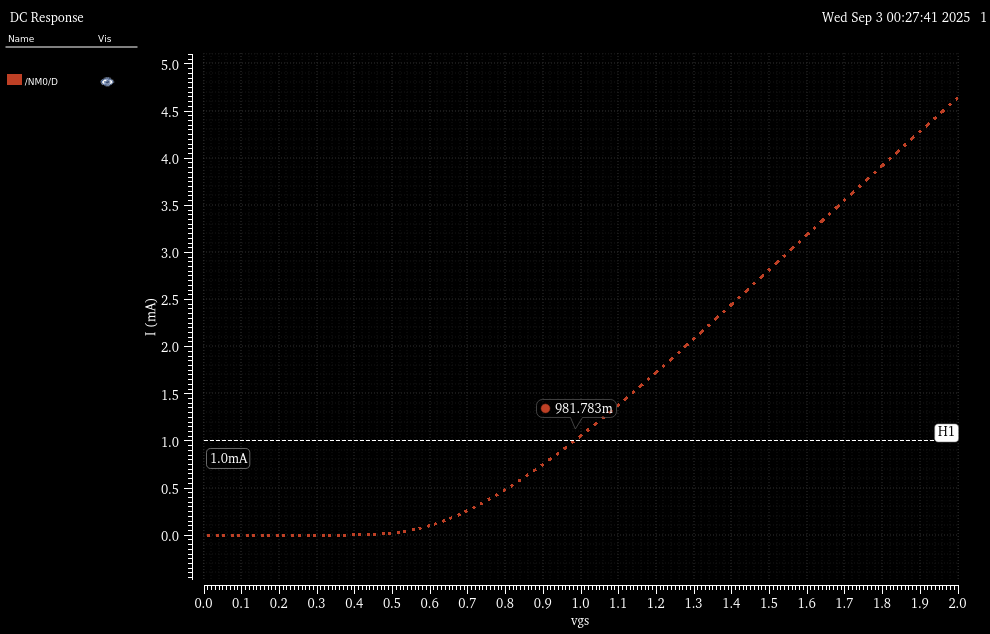
\includegraphics[width=\textwidth]{../Q3b.png}}
	\caption{Width of transistor doubled from fig. \ref{fig:q3a}:
  $W = 12\mu m, L = 0.48\mu m$; simulation re-run with same parameters}
	\label{fig:q3c}
\end{figure}

After doubling just the width of the transistor:

$$
V_{gs} = 0.981783V 
$$

$$
	V_{eff2} = V_{gs} - V_{th} = 0.981783V -  0.489051V = 0.492732V
$$


\subsection*{3c}
After doubling only the width of the transistor, the effective voltage seems to have been halved.
As the transistor is wider, less input voltage is required to reach the same level of current at the drain.

\end{document}